\section{Consensus layer support} \label{sec.consensus}

%\subsection{The interlink pointers data structure}
\label{sec.interlink}

% \subsection{The interlink pointers data structure}
In order to construct our protocol, we rely on the same \emph{interlink data structure} used by PoPoW~\cite{KLS}. This is an
additional hash-based data structure that is proposed to include in the header of heach block.
The interlink data structure is a skip-list~\cite{skiplist} that makes it efficient for a verifier to process a sparse subset of the blockchain, rather than only consecutive blocks.


Observe that in a
blockchain protocol execution it is expected half of the blocks will be of level
$1$, $1/4$ of the blocks will be of level $2$, $1/8$ will be of level $3$ and
$1/2^\mu$ blocks will be of level $\mu$. In expectation, the number of
superblock levels of a chain $\chain$ will be $\Theta(\log(\chain))$~\cite{KLS}.
Figure~\ref{fig.hierarchy} illustrates the blockchain superblocks starting from
level $1$ and going up to level $4$ in case these blocks are distributed exactly
according to expectation. Here, each level contains half the blocks of the level
below.

In our protocol, the verifier must roughly scan along one level at a time.
To enable this,
instead of just the previous block, the interlink vector also points to
the most recent preceding block of every level $\mu$.
Genesis is of infinite level and hence a pointer to it
is included in every block at the first available index within the interlink
data structure. The number of pointers that need
to be included per block is in expectation $\log(|\chain|)$.

\begin{figure}
    \caption{The hierarchical blockchain.
    Higher levels have achieved a lower target (higher difficulty) during mining.}
    \centering
    \iftwocolumn
        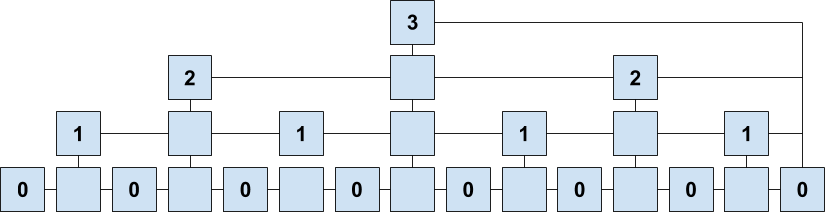
\includegraphics[width=\columnwidth,keepaspectratio]{figures/hierarchical-ledger.png}
    \else
        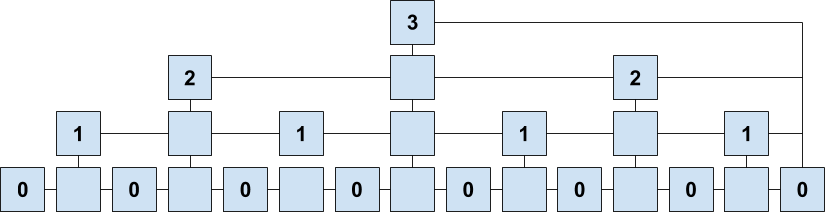
\includegraphics[width=0.7\columnwidth,keepaspectratio]{figures/hierarchical-ledger.png}
    \fi
    \label{fig.hierarchy}
\end{figure}

%The \textit{interlink} data structure is proposed to be included in each block,
%replacing the existing pointer to the previous block with a
%

%\iftr
%The algorithm
%for this construction is shown in Algorithm~\ref{alg.nipopow-interlink} and is
%borrowed from~\cite{KLS}.
%The interlink data structure turns the blockchain into a
%skiplist-like~\cite{skiplist} data structure.

%% The updateInterlink algorithm accepts a block $B'$, which already has an
%% interlink data structure defined on it. The function evaluates the
%% interlink data structure which needs to be included as part of the next block.
%% It copies the existing interlink data structure and
%% then modifies its entries from level $0$ to $\textsf{level}(B')$ to
%% point to the block $B'$.

% \import{./}{algorithms/alg.nipopow-helper.tex}
%\import{./}{algorithms/alg.nipopow-interlink.tex}

% \subsection{Superchain quality}
\noindent{\bf Superchain quality. }
In order to argue formally about the security
properties of blockchains that are equipped with the interlink
data structure we will introduce a new concept of {\em superchain quality},
which generalizes the chain quality property from the backbone model~\cite{backbone}.
We stress that the superchain quality is a new contribution in this paper, and is essential for identifying and overcoming the attack on PoPoW.

We first define a notion of ``goodness'' that bounds the deviation
of superblocks of a certain level from their expected mean. Using
this we then define superchain quality.

It is not hard to see that the above good statistical properties are attained
with overwhelming probability by all chains that are generated in optimistic
environments, i.e. if no adversary tries to violate them.
% \iftr
% \else
We establish the following lemma formally in the full online version.
\begin{lemma}[Optimistic superchain distribution]
\label{lem.superchain-distribution}
For a level $\mu$, and $0 < \delta < 0.5$, a chain
$\chain$ containing only honestly-generated blocks adopted by an honest party in
an execution with random scheduling is $(\delta, m)$-good at level
$\mu$ with overwhelming probability in $m$.
\end{lemma}
%\ fi
